\chapter{Results}%
\label{chap:Results}

In this chapter, the results gathered from our evaluation of the dynamic window against 
the tumbling window will be discussed by the order of the workloads. The workload 
evaluations are run multiple times for consistency of results. We will first 
discuss the workload for latency measurement, followed by periodic workload and 
finally the completeness measurement. For each workload results, we elaborate 
and discuss in details the shortcomings of the evaluation methods and the 
possible outlier situations for which the evaluation result would not agree with.



\section{Workload for latency measurement}%
\label{sec:Results Workload for latency measurement}

This workload is run with a constant low stream rate to ensure that 
the RMLStreamer is not overloaded for a more accurate latency measurement. We also measured 
CPU, throughput, and relative memory usage to determine the improvement brought by Dynamic window
in an ideal streaming environment.

For latency, Tumbling window has a median value of 1915ms, with latency ranging from 1081ms to 2624ms. 
This is as expected since the window is measured using the \emph{average} latency of all records used 
in the joined result at every \emph{trigger} event, which is fired every 2 seconds (the size of tumbling window).
In contrast, Dynamic window has sub second latency with median 57ms and ranging from 39ms to 120ms. Clearly, 
our improvement to fire the \emph{trigger} event whenever a new record arrives inside the subwindow, allows 
Dynamic window to achieve sub second latency. 

Just like latency, the throughput difference between the two windows is also significant. Dynamic window has a 
steady throughput of around 4280 records per second whereas Tumbling window fluctuates around 
3180 and 3240 records per second before stabilizing at 3205 records per second. This is expected as Dynamic 
window eventually stabilizes to a window size processing more records than Tumbling window. This is 
due to adjustment of window sizes at the subwindow level allowing Dynamic window to wait for more records 
with infrequent \emph{key} attribute in the stream before evicting the subwindow. In contrast, Tumbling window 
always evicts the content of the window after 2 seconds, even if it means that there might be more 
eligible records to be joined with the records in the soon to be evicted window, leading to lower throughput.  

Relative memory usage of Dynamic window compared to Tumbling window is similar over the lifetime of the 
evaluation run (Figure~\ref{fig:constant_mem_diff}). Dynamic window causes infrequent \emph{spikes} in memory of more 
than 100 MB memory usage than Tumbling window at certain point in the lifetime of evaluation. This can be attributed 
to the subwindows of Dynamic window growing larger than Tumbling window due to not enough records of the same 
\emph{key} attributes arriving inside the subwindows. However, Dynamic window stabilizes to a more optimal 
window size, where it uses less memory than Tumbling windows, over longer stretches of the evaluation run. At worst case, 
it uses as much memory as Tumbling window does over the course of the evaluation. 

CPU usage is higher by around 7\% for Dynamic window since it requires extra processing of the calculation of metrics. However, this 
increase in CPU usage can also be attributed to the increase in throughput, where the RMLStreamer has more joined results 
to process and map to RDF data.  

\begin{figure*}
    \begin{subfigure}[b]{0.5\textwidth}
        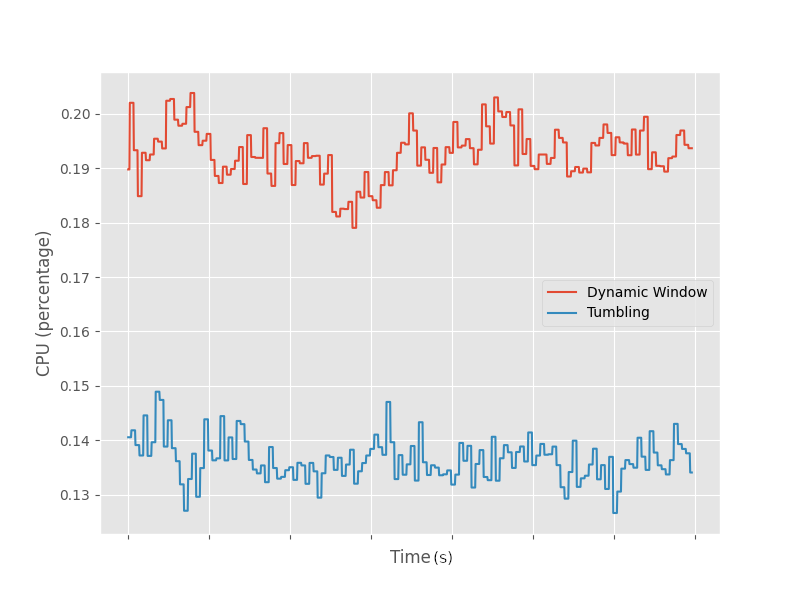
\includegraphics[width=\textwidth]{fig/constant-rate/cpu_comparison.png}
        \caption{CPU usage}
        \label{fig:constant_cpu}
    \end{subfigure}
    \hfill 
    \begin{subfigure}[b]{0.5\textwidth}
        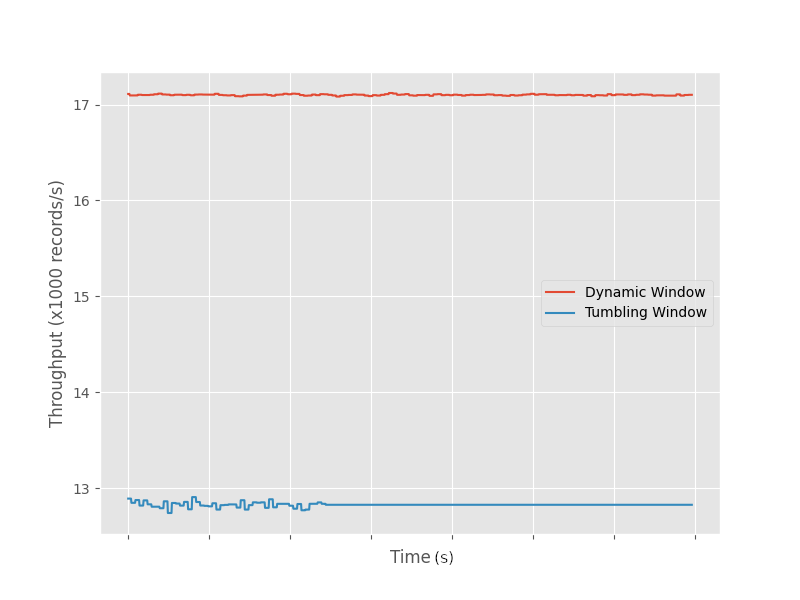
\includegraphics[width=\textwidth]{fig/constant-rate/throughput_comparison.png}
        \caption{Throughput of joined records}
        \label{fig:constant_thorughput}
    \end{subfigure}
    %%
    \begin{subfigure}[b]{0.5\textwidth}
        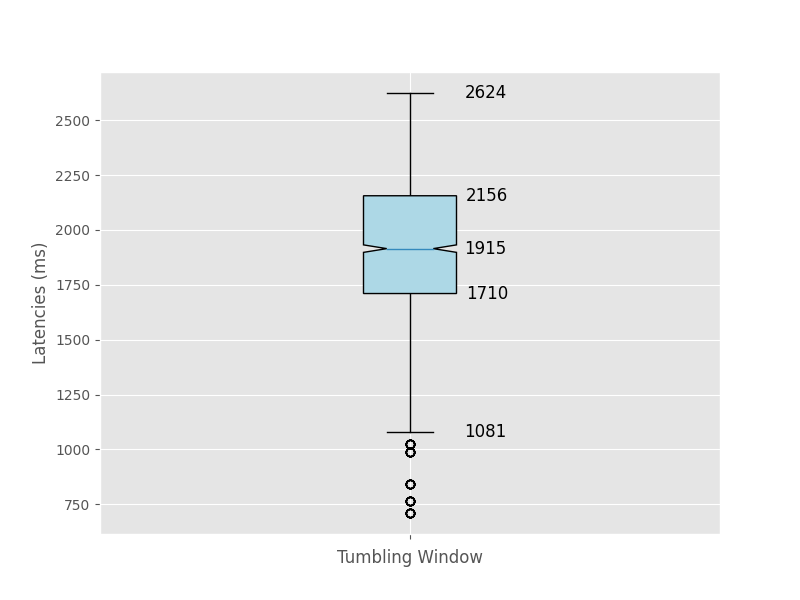
\includegraphics[width=\textwidth]{fig/constant-rate/TumblingWindow_latency_boxplot.png}
        \caption{Tumbling latency}
        \label{fig:constant_tumb_boxplot}
    \end{subfigure}
    \hfill 
    \begin{subfigure}[b]{0.5\textwidth}
        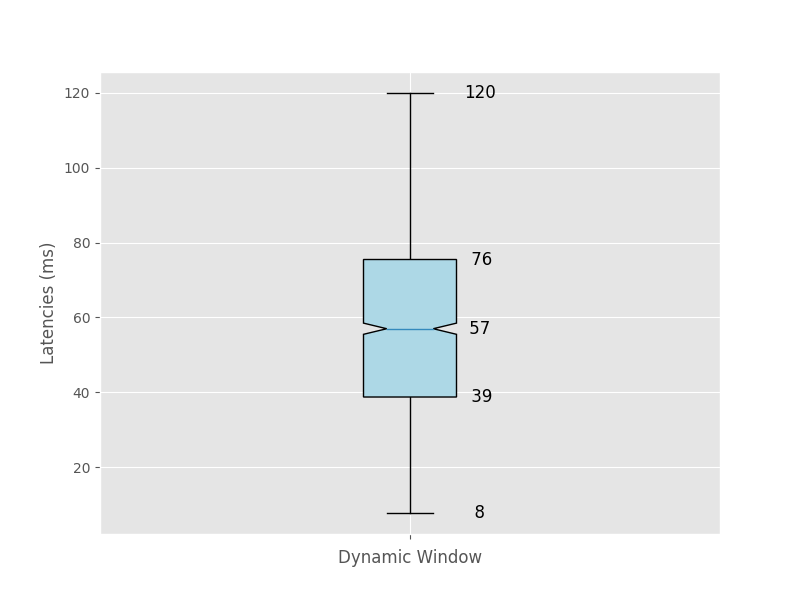
\includegraphics[width=\textwidth]{fig/constant-rate/DynamicWindow_latency_boxplot.png}
        \caption{Dynamic latency}
        \label{fig:constant_dynamic_boxplot}
    \end{subfigure}
    % 
    \begin{subfigure}[b]{\textwidth}
        \centering
        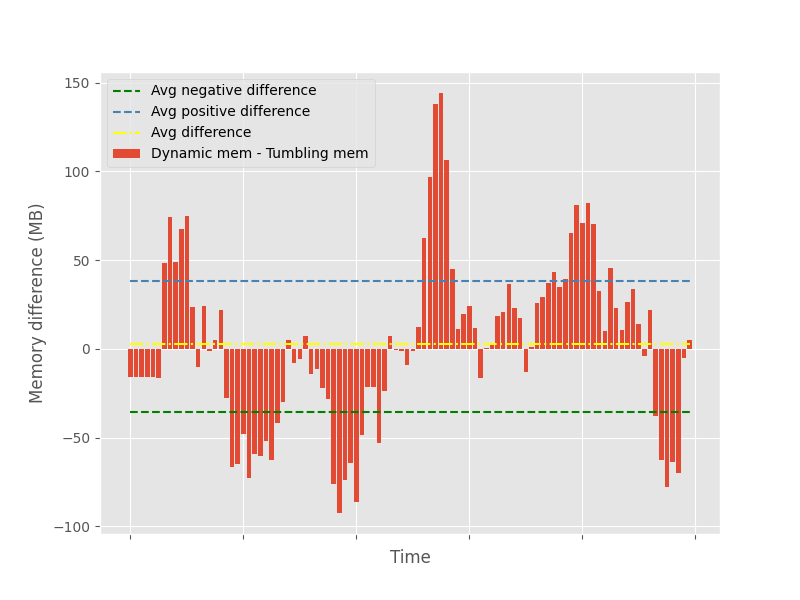
\includegraphics[width=0.5\textwidth]{fig/constant-rate/mem_difference_bar.png}
        \caption{Relative difference in memory usage from the perspective of dynamic window}
        \label{fig:constant_mem_diff}
    \end{subfigure}

    \caption{Metrics measurements for latency workload.}%
    \label{fig:constant_measurement}
\end{figure*}

\section{Workload for periodic burst}%
\label{sec:Results Workload for periodic burst}

Dynamic window still handles the periodic burst of data with lower latency 
than Tumbling window. However, due to the initial size of 2s window updated every 2s, 
the subwindow sizes will grow first until its \textbf{larger} than 2s. This results 
in a temporary increase in latency when the burst of data arrives at the 10th second as 
it is evident in Figure~\ref{fig:periodic_dynamic_lineplot} at the beginning. However, 
Dynamic window manages to shorten the subwindow sizes, with the increase in the stream rate.
This lowers the latency until it is comparable to the latency achieved in the constant stream rate from the 
previous workload.   


\begin{figure*}
    \begin{subfigure}[b]{0.5\textwidth}
        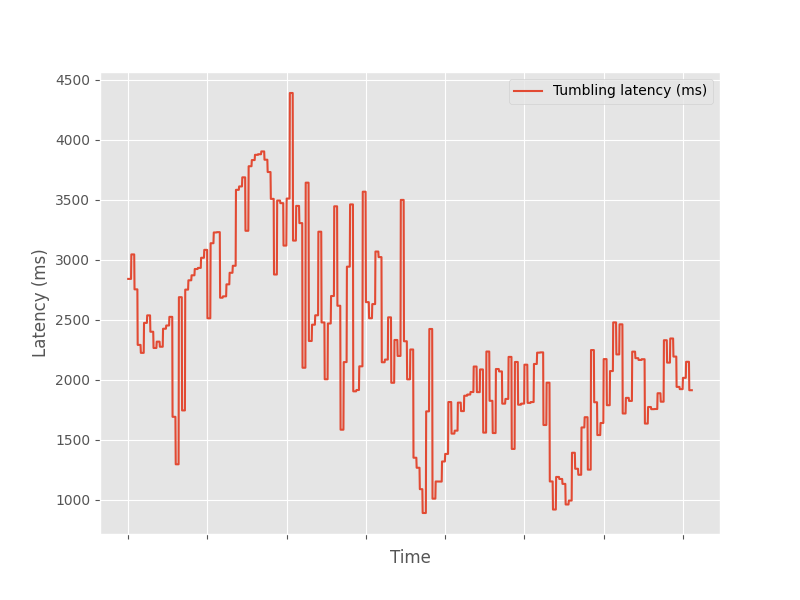
\includegraphics[width=\textwidth]{fig/periodic/Tumbling_latency_lineplot.png}
        \caption{Tumbling latency }
        \label{fig:periodic_tumbling_lineplot}
    \end{subfigure}
    \hfill
    \begin{subfigure}[b]{0.5\textwidth}
        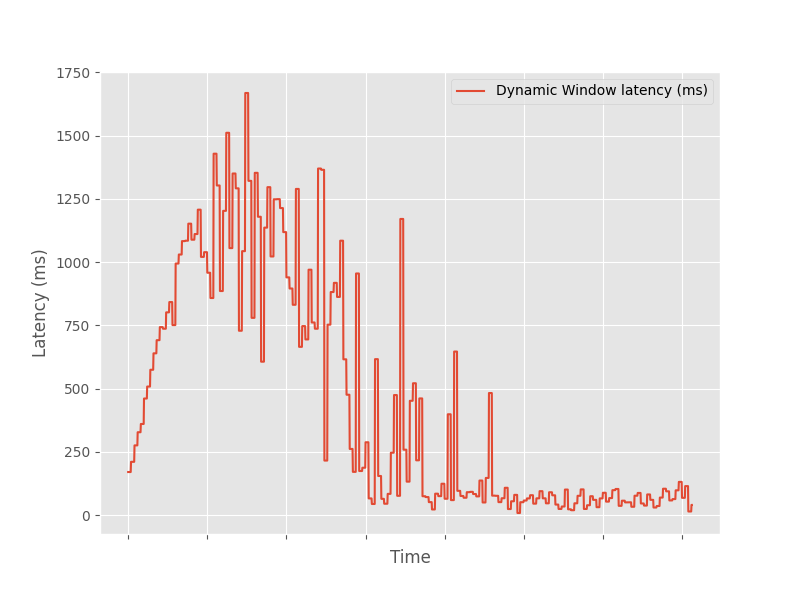
\includegraphics[width=\textwidth]{fig/periodic/DynamicWindow_latency_lineplot.png}
        \caption{Dynamic latency }
        \label{fig:periodic_dynamic_lineplot}
    \end{subfigure}
    \caption{Latency measurement of periodic workload over the lifetime of evaluation}
    \label{fig:periodic_latency_lineplot}
\end{figure*}


\begin{figure*}
    \begin{subfigure}[b]{0.5\textwidth}
        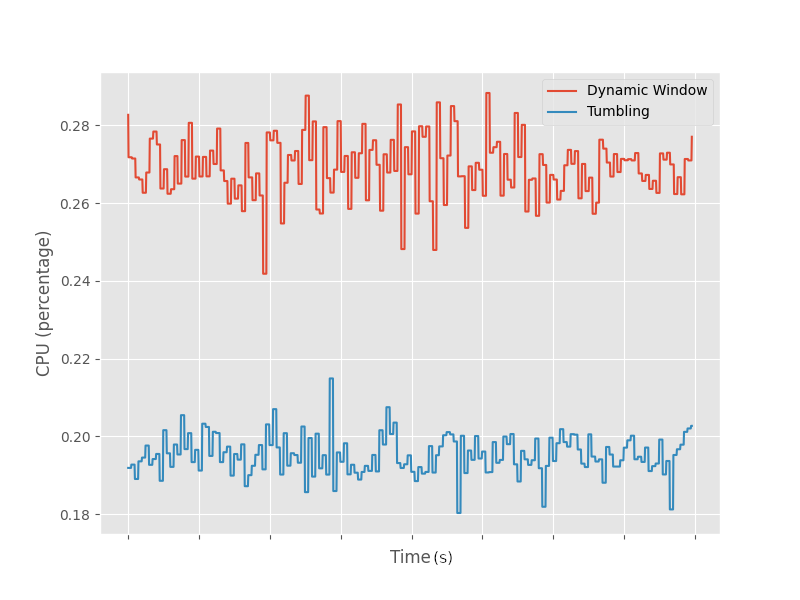
\includegraphics[width=\textwidth]{fig/periodic/cpu_comparison.png}
        \caption{CPU usage}
        \label{fig:periodic_cpu}
    \end{subfigure}
    \hfill 
    \begin{subfigure}[b]{0.5\textwidth}
        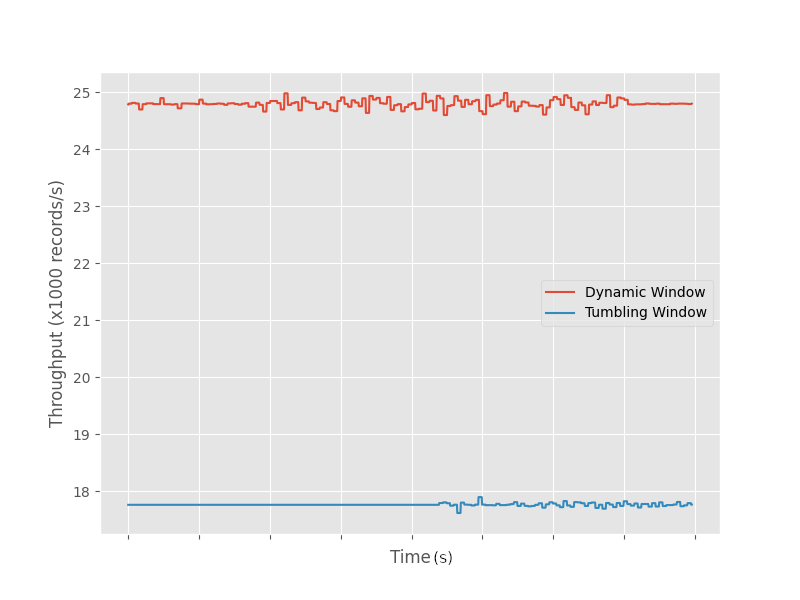
\includegraphics[width=\textwidth]{fig/periodic/throughput_comparison.png}
        \caption{Throughput of joined records}
        \label{fig:periodic_throughput}
    \end{subfigure}
    %%
    \begin{subfigure}[b]{0.5\textwidth}
        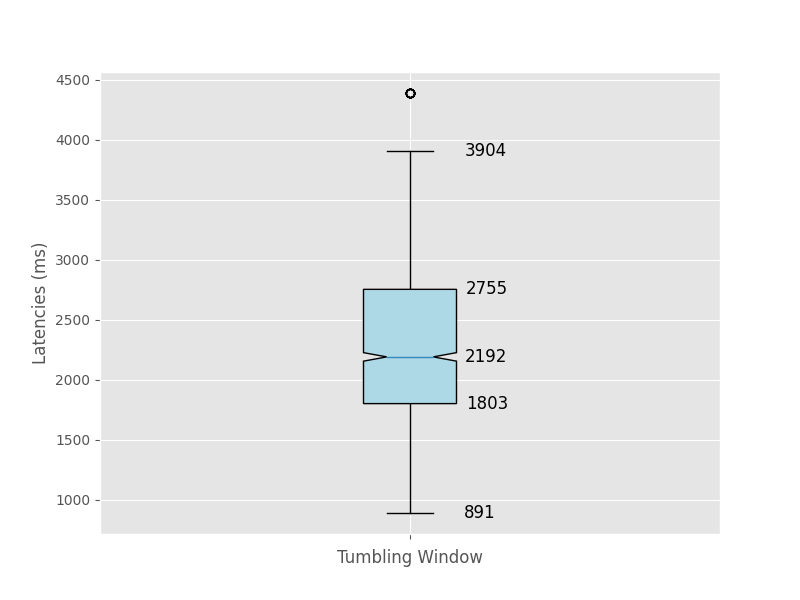
\includegraphics[width=\textwidth]{fig/periodic/TumblingWindow_latency_boxplot.png}
        \caption{Tumbling latency distribution}
        \label{fig:periodic_tumb_boxplot}
    \end{subfigure}
    \hfill 
    \begin{subfigure}[b]{0.5\textwidth}
        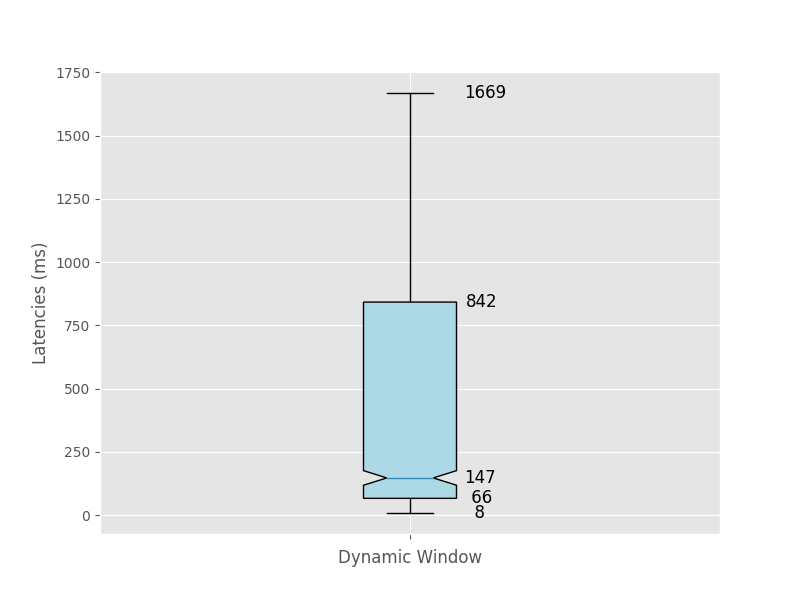
\includegraphics[width=\textwidth]{fig/periodic/DynamicWindow_latency_boxplot.png}
        \caption{Dynamic latency distribution}
        \label{fig:periodic_dynamic_boxplot}
    \end{subfigure}
    % 
    \begin{subfigure}[b]{\textwidth}
        \centering
        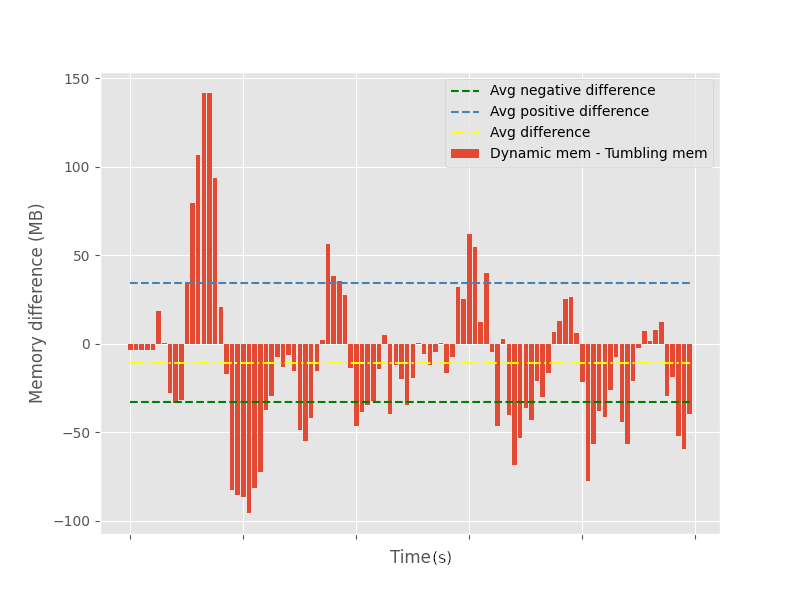
\includegraphics[width=0.5\textwidth]{fig/periodic/mem_difference_bar.png}
        \caption{Relative difference in memory usage from the perspective of dynamic window}
        \label{fig:periodic_mem_diff}
    \end{subfigure}

    \caption{Metrics measurements for periodic workload.}%
    \label{fig:periodic_measurement}
\end{figure*}
